\PassOptionsToPackage{unicode=true}{hyperref} % options for packages loaded elsewhere
\PassOptionsToPackage{hyphens}{url}
%
\documentclass[ignorenonframetext,]{beamer}
\usepackage{pgfpages}
\setbeamertemplate{caption}[numbered]
\setbeamertemplate{caption label separator}{: }
\setbeamercolor{caption name}{fg=normal text.fg}
\beamertemplatenavigationsymbolsempty
% Prevent slide breaks in the middle of a paragraph:
\widowpenalties 1 10000
\raggedbottom
\setbeamertemplate{part page}{
\centering
\begin{beamercolorbox}[sep=16pt,center]{part title}
  \usebeamerfont{part title}\insertpart\par
\end{beamercolorbox}
}
\setbeamertemplate{section page}{
\centering
\begin{beamercolorbox}[sep=12pt,center]{part title}
  \usebeamerfont{section title}\insertsection\par
\end{beamercolorbox}
}
\setbeamertemplate{subsection page}{
\centering
\begin{beamercolorbox}[sep=8pt,center]{part title}
  \usebeamerfont{subsection title}\insertsubsection\par
\end{beamercolorbox}
}
\AtBeginPart{
  \frame{\partpage}
}
\AtBeginSection{
  \ifbibliography
  \else
    \frame{\sectionpage}
  \fi
}
\AtBeginSubsection{
  \frame{\subsectionpage}
}
\usepackage{lmodern}
\usepackage{amssymb,amsmath}
\usepackage{ifxetex,ifluatex}
\usepackage{fixltx2e} % provides \textsubscript
\ifnum 0\ifxetex 1\fi\ifluatex 1\fi=0 % if pdftex
  \usepackage[T1]{fontenc}
  \usepackage[utf8]{inputenc}
  \usepackage{textcomp} % provides euro and other symbols
\else % if luatex or xelatex
  \usepackage{unicode-math}
  \defaultfontfeatures{Ligatures=TeX,Scale=MatchLowercase}
\fi
% use upquote if available, for straight quotes in verbatim environments
\IfFileExists{upquote.sty}{\usepackage{upquote}}{}
% use microtype if available
\IfFileExists{microtype.sty}{%
\usepackage[]{microtype}
\UseMicrotypeSet[protrusion]{basicmath} % disable protrusion for tt fonts
}{}
\IfFileExists{parskip.sty}{%
\usepackage{parskip}
}{% else
\setlength{\parindent}{0pt}
\setlength{\parskip}{6pt plus 2pt minus 1pt}
}
\usepackage{hyperref}
\hypersetup{
            pdftitle={Random Numbers in R},
            pdfauthor={Hans W Borchers},
            pdfborder={0 0 0},
            breaklinks=true}
\urlstyle{same}  % don't use monospace font for urls
\newif\ifbibliography
\usepackage{color}
\usepackage{fancyvrb}
\newcommand{\VerbBar}{|}
\newcommand{\VERB}{\Verb[commandchars=\\\{\}]}
\DefineVerbatimEnvironment{Highlighting}{Verbatim}{commandchars=\\\{\}}
% Add ',fontsize=\small' for more characters per line
\usepackage{framed}
\definecolor{shadecolor}{RGB}{248,248,248}
\newenvironment{Shaded}{\begin{snugshade}}{\end{snugshade}}
\newcommand{\AlertTok}[1]{\textcolor[rgb]{0.94,0.16,0.16}{#1}}
\newcommand{\AnnotationTok}[1]{\textcolor[rgb]{0.56,0.35,0.01}{\textbf{\textit{#1}}}}
\newcommand{\AttributeTok}[1]{\textcolor[rgb]{0.77,0.63,0.00}{#1}}
\newcommand{\BaseNTok}[1]{\textcolor[rgb]{0.00,0.00,0.81}{#1}}
\newcommand{\BuiltInTok}[1]{#1}
\newcommand{\CharTok}[1]{\textcolor[rgb]{0.31,0.60,0.02}{#1}}
\newcommand{\CommentTok}[1]{\textcolor[rgb]{0.56,0.35,0.01}{\textit{#1}}}
\newcommand{\CommentVarTok}[1]{\textcolor[rgb]{0.56,0.35,0.01}{\textbf{\textit{#1}}}}
\newcommand{\ConstantTok}[1]{\textcolor[rgb]{0.00,0.00,0.00}{#1}}
\newcommand{\ControlFlowTok}[1]{\textcolor[rgb]{0.13,0.29,0.53}{\textbf{#1}}}
\newcommand{\DataTypeTok}[1]{\textcolor[rgb]{0.13,0.29,0.53}{#1}}
\newcommand{\DecValTok}[1]{\textcolor[rgb]{0.00,0.00,0.81}{#1}}
\newcommand{\DocumentationTok}[1]{\textcolor[rgb]{0.56,0.35,0.01}{\textbf{\textit{#1}}}}
\newcommand{\ErrorTok}[1]{\textcolor[rgb]{0.64,0.00,0.00}{\textbf{#1}}}
\newcommand{\ExtensionTok}[1]{#1}
\newcommand{\FloatTok}[1]{\textcolor[rgb]{0.00,0.00,0.81}{#1}}
\newcommand{\FunctionTok}[1]{\textcolor[rgb]{0.00,0.00,0.00}{#1}}
\newcommand{\ImportTok}[1]{#1}
\newcommand{\InformationTok}[1]{\textcolor[rgb]{0.56,0.35,0.01}{\textbf{\textit{#1}}}}
\newcommand{\KeywordTok}[1]{\textcolor[rgb]{0.13,0.29,0.53}{\textbf{#1}}}
\newcommand{\NormalTok}[1]{#1}
\newcommand{\OperatorTok}[1]{\textcolor[rgb]{0.81,0.36,0.00}{\textbf{#1}}}
\newcommand{\OtherTok}[1]{\textcolor[rgb]{0.56,0.35,0.01}{#1}}
\newcommand{\PreprocessorTok}[1]{\textcolor[rgb]{0.56,0.35,0.01}{\textit{#1}}}
\newcommand{\RegionMarkerTok}[1]{#1}
\newcommand{\SpecialCharTok}[1]{\textcolor[rgb]{0.00,0.00,0.00}{#1}}
\newcommand{\SpecialStringTok}[1]{\textcolor[rgb]{0.31,0.60,0.02}{#1}}
\newcommand{\StringTok}[1]{\textcolor[rgb]{0.31,0.60,0.02}{#1}}
\newcommand{\VariableTok}[1]{\textcolor[rgb]{0.00,0.00,0.00}{#1}}
\newcommand{\VerbatimStringTok}[1]{\textcolor[rgb]{0.31,0.60,0.02}{#1}}
\newcommand{\WarningTok}[1]{\textcolor[rgb]{0.56,0.35,0.01}{\textbf{\textit{#1}}}}
\usepackage{graphicx,grffile}
\makeatletter
\def\maxwidth{\ifdim\Gin@nat@width>\linewidth\linewidth\else\Gin@nat@width\fi}
\def\maxheight{\ifdim\Gin@nat@height>\textheight\textheight\else\Gin@nat@height\fi}
\makeatother
% Scale images if necessary, so that they will not overflow the page
% margins by default, and it is still possible to overwrite the defaults
% using explicit options in \includegraphics[width, height, ...]{}
\setkeys{Gin}{width=\maxwidth,height=\maxheight,keepaspectratio}
\setlength{\emergencystretch}{3em}  % prevent overfull lines
\providecommand{\tightlist}{%
  \setlength{\itemsep}{0pt}\setlength{\parskip}{0pt}}
\setcounter{secnumdepth}{0}

% set default figure placement to htbp
\makeatletter
\def\fps@figure{htbp}
\makeatother


\title{Random Numbers in R}
\author{\textbf{Hans W Borchers}}
\date{\emph{Heidelberg, February 2019}}

\begin{document}
\frame{\titlepage}

\hypertarget{random-numbers}{%
\section{Random Numbers}\label{random-numbers}}

\begin{frame}[fragile]{Random Number Generators (RNGs)}
\protect\hypertarget{random-number-generators-rngs}{}

\begin{itemize}
\item
  (\emph{Pseudo}-)Random number generators in Base R

\begin{verbatim}
RNGkind(kind = "default", normal.kind = NULL)
set.seed(seed)  # i.e., seed <- .Random.seed 

runif(n)        # or: rnorm(n); rexp(n)
sample(x, size, replace = FALSE, prob = NULL)
\end{verbatim}

  Wichmann-Hill: \(6.9\cdot10^{12}\); Marsaglia-Multicarry:
  \(1.1\cdot10^{18}\)\\
  Super-Duper: \(4.6\cdot 10^{18}\); \textbf{Mersenne-Twister}:
  \(\approx 10^{6000}\)\\
  Knuth-TAOCP-2002: \(6.8 \cdot 10^{38}\); L'Ecuyer-CMRG:
  \(3.1\cdot 10^{57}\)
\item
  Recommended `help' pages:

\begin{verbatim}
?Random       # details on RNG in R, 'kinds', 'seeds', etc.
?Random.user  # user-supplied random number generation
\end{verbatim}
\end{itemize}

\end{frame}

\begin{frame}[fragile]{dqrng and qrng Packages}
\protect\hypertarget{dqrng-and-qrng-packages}{}

\begin{itemize}
\item
  \textbf{dqrng}: Fast pseudo-random number generator

\begin{verbatim}
dqrunif()`, `dqrnorm()`, `dqrexp()
dqset.seed()`, `dqRNGkind(kind = "Mersenne-Twister")
\end{verbatim}

  64-bit Mersenne-Twister, pcg64,\\
  Xoroshiro128+, Xoshiro256+ (defaults in Erlang and Lua),\\
  Threefry (64 bit engine provided by \textbf{sitmo})
\item
  \textbf{qrng}: \emph{Quasi}-random numbers in high dimensions

\begin{verbatim}
korobov(n, d = 1, generator, randomize = FALSE)
ghalton(n, d = 1, method = c("generalized", "halton"))
sobol  (n, d = 1, randomize = FALSE, skip = 0)
\end{verbatim}

  Developed specifically for Monte-Carlo applications
\end{itemize}

\end{frame}

\begin{frame}{Pseudo, quasi, and true RNGs}
\protect\hypertarget{pseudo-quasi-and-true-rngs}{}

\begin{itemize}
\item
  \emph{Pseudo-random numbers}\\
  are sequences of numbers whose statistical properties approximate the
  properties of theoretical random number sequences.
\item
  \emph{Quasi-random numbers}\\
  are `low-discrepancy sequences', that is the proportion of numbers
  falling into an arbitrary subset is close to the measure of that
  subset.
\item
  \emph{True random numbers}\\
  are generated from physical processes that are known to behave like
  statistically random `noise' signals.
\end{itemize}

\end{frame}

\begin{frame}[fragile]{\emph{True} Random Number Generators}
\protect\hypertarget{true-random-number-generators}{}

\begin{itemize}
\item
  \textbf{random}\\
  RANDOM.ORG ``samples atmospheric noise via radio tuned to an unused
  broadcasting frequency together with a skew correction algorithm by
  John von Neumann.''

\begin{verbatim}
library(random); N = 10000  # maximum request
rn <- randomNumbers(n = N, min = 0, max = N, col = 2)/N
\end{verbatim}
\item
  \textbf{qrandom}\\
  ANU Quantum Random Number Generator ``generates true random numbers in
  real-time by measuring the quantum fluctuations of the vacuum.''

\begin{verbatim}
library(qrandom); N = 10000  # maximum request: 10^5 [1024]
rn <- qrandomunif(n = N, a = 0, b = 1)
\end{verbatim}
\end{itemize}

\end{frame}

\begin{frame}[fragile]{Generate Random Distributions}
\protect\hypertarget{generate-random-distributions}{}

If \(u\) are uniformly distributed random numbers (in \([0, 1]\))\\
and \(F\) is a \emph{cumulative distribution function}, then the
numbers\\
\(F^{-1}(u)\) are random numbers in this statistical distribution.

Example: Normal (Gaussian) distribution\\
( with mean = 0.0 and sd = 1.0)

\begin{Shaded}
\begin{Highlighting}[]
\NormalTok{    x  <-}\StringTok{ }\KeywordTok{runif}\NormalTok{(}\DecValTok{1000}\NormalTok{)}
\NormalTok{    xn <-}\StringTok{ }\KeywordTok{qnorm}\NormalTok{(x)      }\CommentTok{# qnorm() is the inverse of pnorm()}
    \KeywordTok{summary}\NormalTok{(xn)}
\end{Highlighting}
\end{Shaded}

\begin{verbatim}
##     Min.  1st Qu.   Median     Mean  3rd Qu.     Max. 
## -2.83681 -0.68305  0.06580  0.04031  0.72586  2.87980
\end{verbatim}

Alternative: Ziggurat algorithm

\end{frame}

\begin{frame}{More RNGs in Packages}
\protect\hypertarget{more-rngs-in-packages}{}

\begin{itemize}
\item
  \textbf{randaes} (2012)\\
  cryptographic random number generator, based on AES
\item
  \textbf{rngwell19937} (2014)\\
  long period linear random number generator WELL19937a
\item
  \textbf{rstream} (2017)\\
  streams of random numbers from different sources
\item
  \textbf{Tinflex} (2017)\\
  generator for arbitrary distributions with piecewise\\
  twice differentiable densities
\item
  \textbf{UnivRNG} and \textbf{MultiRNG} (2018)\\
  uni-/multivariate random number generation for quite\\
  a number of different distributions
\end{itemize}

\end{frame}

\begin{frame}[fragile]{User-defined RNGs and Tools}
\protect\hypertarget{user-defined-rngs-and-tools}{}

\begin{itemize}
\item
  \emph{?Random.user}\\
  ``Function \texttt{RNGkind()} allows user-coded uniform and normal
  random number generators to be supplied.''

\begin{verbatim}
dyn.load("<user.lib>")
RNGkind(kind = "user-supplied")
\end{verbatim}
\item
  \textbf{randtoolbox}\\
  Toolbox for pseudo and quasi random number generation
\item
  \textbf{rngtools}\\
  Utility functions for working with RNGs
\item
  \textbf{setRNG}\\
  for compatibility with former S versions
\end{itemize}

\end{frame}

\begin{frame}[fragile]{How to Write your own RNG in R?}
\protect\hypertarget{how-to-write-your-own-rng-in-r}{}

\begin{itemize}
\item
  Congruential random number generation

  \[x_{i+1} = (a x_i + c)\,\mathrm{mod}\,m\]

\begin{verbatim}
e.g., m = 2^32,     a = 1103515245, c = 12345
or    m = 2^31 - 1, a = 48271,      c = 0     (Lehmer RNGs)
\end{verbatim}
\item
  Knuth-TAOCP-2002

  \[x_i = (x_{i-37} + x_{i-100})\,\mathrm{mod}\,2^{30}\] (and discard
  the first 2000 numbers)
\end{itemize}

See also the \textbf{randtoolbox} vignette, Dutang and Würtz (2009)\\
\emph{A note on random number generation}

\end{frame}

\begin{frame}[fragile]

\textbf{Knuth-TAOCP-2002} -- an R Implementation

\begin{verbatim}
randTAOCP <- function(seed = NULL) {
    local({
        R <- vector(mode = "numeric", length = 2000)
        R[1:100] <- qrandom::qrandomunif(n = 100, a = 0, b = 1)
        for (k in 101:2000)
            R[k] <- (R[k-37] + R[k-100]) %% 1
        k <- 2000; i <- 2000 - 37; j <- 2000 - 100
        frand <- function() {
            k <<- (k %% 2000) + 1
            i <<- (i %% 2000) + 1
            j <<- (j %% 2000) + 1
            z <- (R[i] + R[j]) %% 1
            R[k] <<- z
            return(z)
        }
        return(frand)
    })
}
\end{verbatim}

\end{frame}

\hypertarget{tests-for-rngs}{%
\section{Tests for RNGs}\label{tests-for-rngs}}

\begin{frame}{Testing Random Number Generators}
\protect\hypertarget{testing-random-number-generators}{}

\begin{itemize}
\item
  \textbf{RDieHarder}\\
  R Interface to the `DieHarder' RNG Test Suite

  Not even `Mersenne Twister' satisfies all these tests!
\item
  Simple RNG tests, e.g.

  \begin{itemize}
  \item
    Spectral test in d dimensions
  \item
    Permutation rank distribution
  \item
    Monte Carlo value for \(\pi\)
  \item
    `Greatest Common Divisor' test
  \item
    Birthday spacing test
  \item
    \emph{Random Walk} tests
  \end{itemize}
\end{itemize}

\end{frame}

\begin{frame}{Example: 3D Spectral Test}
\protect\hypertarget{example-3d-spectral-test}{}

Search for lattice structure (in all dimensions)

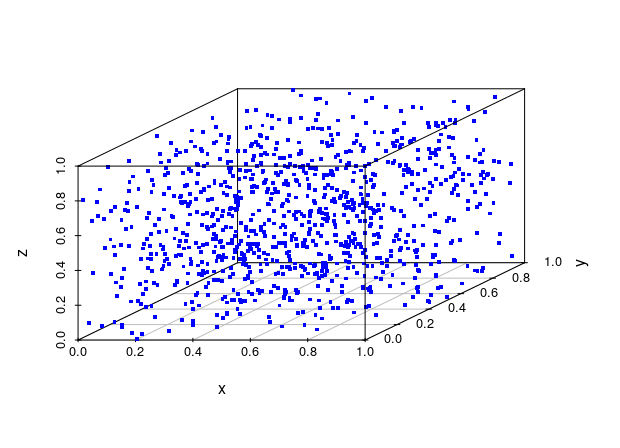
\includegraphics{test.png}

\end{frame}

\begin{frame}{Example: Image Sampling}
\protect\hypertarget{example-image-sampling}{}

Mitchell's best-candidate algorithm for Poisson disk distribution

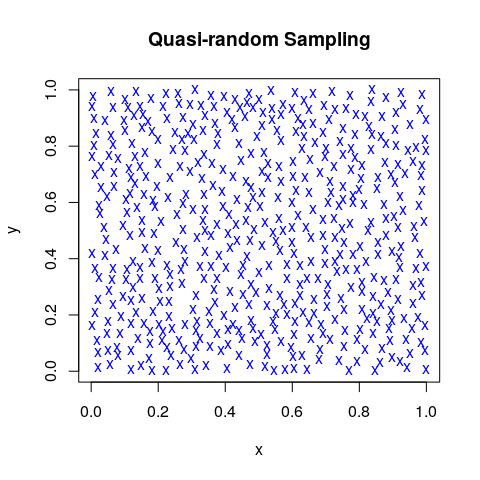
\includegraphics{quasirandom.png}

\end{frame}

\hypertarget{example-random-walks}{%
\section{Example: Random Walks}\label{example-random-walks}}

\begin{frame}{``Irrfahrten und ihre Folgen''}
\protect\hypertarget{irrfahrten-und-ihre-folgen}{}

\textbf{Definition} (Pearson 1905)\\
A \textbf{random walk} consists of a succession of random steps on some
discrete grid. An elementary example is the \textbf{symmetric} random
walk on the integers that starts at 0 and at each step moves +1 or −1
with equal probability.

\textbf{Theorem} (Polya 1921).\\
\emph{A symmetric random walk in one or two dimensions will return\\
to its starting point} almost certainly \emph{(i.e., with probability
1)}.

Applications in\\
Queing models, Brownian motion, stock markets, animal behavior, risk
analysis, diffusion processes, game theory, \ldots{}

Random walks are fundamental for Markov processes.

\end{frame}

\begin{frame}{Visualization of Random Walks}
\protect\hypertarget{visualization-of-random-walks}{}

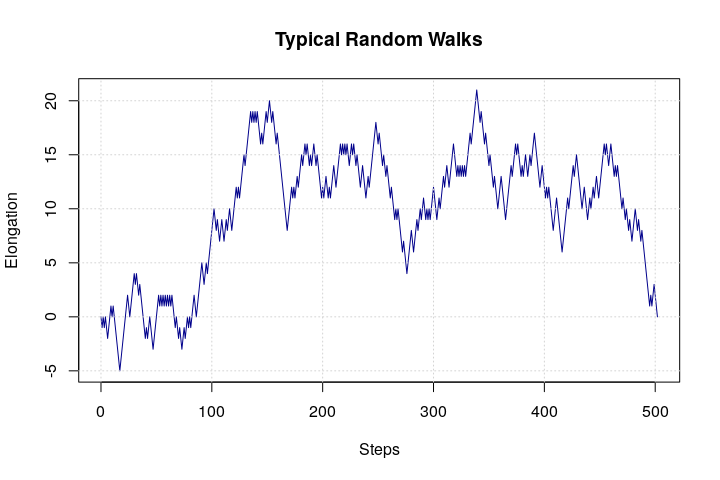
\includegraphics{TypRandomWalks.png}

\end{frame}

\begin{frame}{Original Project Idea}
\protect\hypertarget{original-project-idea}{}

\textbf{Goal}

\begin{itemize}
\tightlist
\item
  Generate a million or so example curves, starting and ending\\
  in 0, by smoothing enough random walks (splines, etc.)
\item
  Store these curves in appropriate databases
\item
  Apply \textbf{Functional Data Analysis} (FDA) methods to classify,
  compare by similarity, and retrieve similar curves
\end{itemize}

\textbf{Problem}

\begin{itemize}
\item
  Find enough nontrivial random walks returning to 0
\item
  \textbf{Or}: What is the probability that a random walk returns to 0
  after at most \emph{n} steps?
\end{itemize}

\end{frame}

\begin{frame}[fragile]{Random Walks Step-by-Step}
\protect\hypertarget{random-walks-step-by-step}{}

\begin{Shaded}
\begin{Highlighting}[]
\NormalTok{rwalk <-}\StringTok{ }\ControlFlowTok{function}\NormalTok{(N, M) \{}
\NormalTok{    result <-}\StringTok{ }\KeywordTok{rep}\NormalTok{(}\DecValTok{0}\NormalTok{, N)}
    \ControlFlowTok{for}\NormalTok{ (i }\ControlFlowTok{in} \DecValTok{1}\OperatorTok{:}\NormalTok{N) \{}
\NormalTok{        steps <-}\StringTok{ }\DecValTok{2}
\NormalTok{        a <-}\StringTok{ }\ControlFlowTok{if}\NormalTok{ (}\KeywordTok{dqrunif}\NormalTok{(}\DecValTok{1}\NormalTok{) }\OperatorTok{>=}\StringTok{ }\FloatTok{0.5}\NormalTok{) }\DecValTok{1} \ControlFlowTok{else} \DecValTok{-1}
\NormalTok{        a <-}\StringTok{ }\NormalTok{a }\OperatorTok{+}\StringTok{ }\ControlFlowTok{if}\NormalTok{ (}\KeywordTok{dqrunif}\NormalTok{(}\DecValTok{1}\NormalTok{) }\OperatorTok{>=}\StringTok{ }\FloatTok{0.5}\NormalTok{) }\DecValTok{1} \ControlFlowTok{else} \DecValTok{-1}
        \ControlFlowTok{while}\NormalTok{ (a }\OperatorTok{!=}\StringTok{ }\DecValTok{0}\NormalTok{) \{}
\NormalTok{            steps <-}\StringTok{ }\NormalTok{steps }\OperatorTok{+}\StringTok{ }\DecValTok{2}
\NormalTok{            a <-}\StringTok{ }\NormalTok{a }\OperatorTok{+}\StringTok{ }\ControlFlowTok{if}\NormalTok{ (}\KeywordTok{dqrunif}\NormalTok{(}\DecValTok{1}\NormalTok{) }\OperatorTok{>=}\StringTok{ }\FloatTok{0.5}\NormalTok{) }\DecValTok{1} \ControlFlowTok{else} \DecValTok{-1}
\NormalTok{            a <-}\StringTok{ }\NormalTok{a }\OperatorTok{+}\StringTok{ }\ControlFlowTok{if}\NormalTok{ (}\KeywordTok{dqrunif}\NormalTok{(}\DecValTok{1}\NormalTok{) }\OperatorTok{>=}\StringTok{ }\FloatTok{0.5}\NormalTok{) }\DecValTok{1} \ControlFlowTok{else} \DecValTok{-1}
            \ControlFlowTok{if}\NormalTok{ (steps }\OperatorTok{>=}\StringTok{ }\NormalTok{M) }\ControlFlowTok{break}
\NormalTok{        \}}
\NormalTok{        result[i] <-}\StringTok{ }\NormalTok{steps}
\NormalTok{    \}}
\NormalTok{    result}
\NormalTok{\}}
\end{Highlighting}
\end{Shaded}

Discussion on other, more compact approaches ?

\end{frame}

\begin{frame}{Probability Distribution of RWs}
\protect\hypertarget{probability-distribution-of-rws}{}

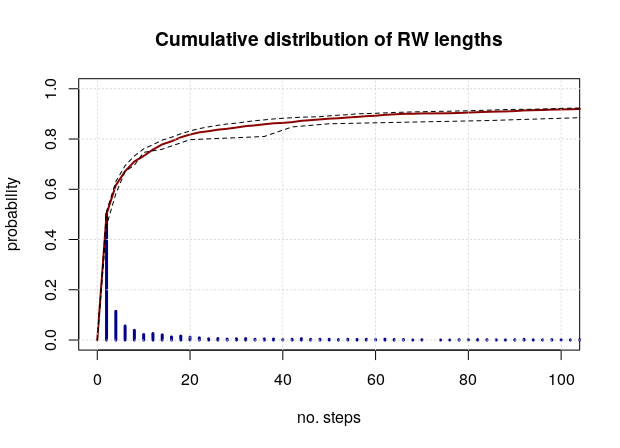
\includegraphics{cumprob.png}

\end{frame}

\begin{frame}[fragile]{Derive Minimum No.~of Steps}
\protect\hypertarget{derive-minimum-no.of-steps}{}

\begin{Shaded}
\begin{Highlighting}[]
\NormalTok{N <-}\StringTok{ }\DecValTok{10000}\NormalTok{; M =}\StringTok{ }\DecValTok{2048}
\NormalTok{result <-}\StringTok{ }\KeywordTok{numeric}\NormalTok{(}\DecValTok{100}\NormalTok{)}
\ControlFlowTok{for}\NormalTok{ (i }\ControlFlowTok{in} \DecValTok{1}\OperatorTok{:}\DecValTok{100}\NormalTok{) \{              }\CommentTok{# 100 simulation runs}
\NormalTok{    no_steps <-}\StringTok{ }\KeywordTok{rwalk}\NormalTok{(N, M)     }\CommentTok{# vector of step lengths}
\NormalTok{    r <-}\StringTok{ }\KeywordTok{rle}\NormalTok{(}\KeywordTok{sort}\NormalTok{(no_steps))    }\CommentTok{# 'run length encoding'}
\NormalTok{    x <-}\StringTok{ }\NormalTok{r}\OperatorTok{$}\NormalTok{values               }\CommentTok{# steps}
\NormalTok{    y <-}\StringTok{ }\KeywordTok{cumsum}\NormalTok{(r}\OperatorTok{$}\NormalTok{lengths)}\OperatorTok{/}\NormalTok{N    }\CommentTok{# probability}
\NormalTok{    ind <-}\StringTok{ }\KeywordTok{which}\NormalTok{(y }\OperatorTok{>}\StringTok{ }\FloatTok{0.975}\NormalTok{)[}\DecValTok{1}\NormalTok{]  }\CommentTok{# where is p > 0.975}
\NormalTok{    result[i] <-}\StringTok{ }\NormalTok{x[ind]         }\CommentTok{# store no. of steps}
\NormalTok{\}}

\KeywordTok{summary}\NormalTok{(result)}
\CommentTok{##  ...}
\end{Highlighting}
\end{Shaded}

Repeat this for different uniform RNGs in \texttt{rwalk()}

\end{frame}

\begin{frame}[fragile]{Simulation Results}
\protect\hypertarget{simulation-results}{}

Simulate 100 times and compute the 97.5\% level:\\
10000 random walks -- stopping at length 2048

\begin{verbatim}
# with `runif()`
> summary(result)
##  Min. 1st Qu.  Median    Mean 3rd Qu.    Max.
##   684     959    1018    1038    1120    1476

# with `dqrunif()`
> summary(result)
##  Min. 1st Qu.  Median    Mean 3rd Qu.    Max.
##   752     941    1013    1025    1108    1320

# with `randTAoCP()`
> summary(result)
##  Min. 1st Qu.  Median    Mean 3rd Qu.    Max. 
##   806     944    1003    1026    1098    1302 
\end{verbatim}

\end{frame}

\begin{frame}[fragile]{Theory of Random Walks}
\protect\hypertarget{theory-of-random-walks}{}

The probability for returning to zero for the first time after exactly
2n steps is:
\[P(W = 2n) = {2(n-1) \choose n-1} \frac{1}{2^{2(n-1)}} \frac{1}{2n}\]

\begin{Shaded}
\begin{Highlighting}[]
\NormalTok{n <-}\StringTok{ }\DecValTok{1}\OperatorTok{:}\DecValTok{512}
\NormalTok{a <-}\StringTok{ }\KeywordTok{choose}\NormalTok{(}\DecValTok{2}\OperatorTok{*}\NormalTok{(n}\DecValTok{-1}\NormalTok{), n}\DecValTok{-1}\NormalTok{)}\OperatorTok{/}\DecValTok{2}\OperatorTok{^}\NormalTok{(}\DecValTok{2}\OperatorTok{*}\NormalTok{(n}\DecValTok{-1}\NormalTok{))}\OperatorTok{/}\NormalTok{(}\DecValTok{2}\OperatorTok{*}\NormalTok{n)}
\NormalTok{w <-}\StringTok{ }\KeywordTok{c}\NormalTok{(}\DecValTok{0}\NormalTok{, }\KeywordTok{cumsum}\NormalTok{(a))}
\KeywordTok{cbind}\NormalTok{(}\DecValTok{2}\OperatorTok{*}\KeywordTok{c}\NormalTok{(}\DecValTok{510}\OperatorTok{:}\DecValTok{512}\NormalTok{), w[}\DecValTok{510}\OperatorTok{:}\DecValTok{512}\NormalTok{])}
\end{Highlighting}
\end{Shaded}

\begin{verbatim}
##      [,1]      [,2]
## [1,] 1020 0.9749989
## [2,] 1022 0.9750234
## [3,] 1024 0.9750478
\end{verbatim}

\end{frame}

\begin{frame}[fragile]{Remark about the \(P = 0.99\) Case}
\protect\hypertarget{remark-about-the-p-0.99-case}{}

\texttt{choose()} does not work for bigger numbers.\\
We need to aply the `arbitrary-precision' package \textbf{gmp}.

\begin{Shaded}
\begin{Highlighting}[]
\NormalTok{n <-}\StringTok{ }\DecValTok{1}\OperatorTok{:}\DecValTok{3185}
\NormalTok{b2 <-}\StringTok{ }\KeywordTok{as.bigz}\NormalTok{(}\DecValTok{2}\NormalTok{)}
\NormalTok{A <-}\StringTok{ }\KeywordTok{chooseZ}\NormalTok{(b2}\OperatorTok{*}\NormalTok{(n}\DecValTok{-1}\NormalTok{), n}\DecValTok{-1}\NormalTok{)}\OperatorTok{/}\NormalTok{(b2}\OperatorTok{^}\NormalTok{(b2}\OperatorTok{*}\NormalTok{(n}\DecValTok{-1}\NormalTok{))}\OperatorTok{*}\NormalTok{(b2}\OperatorTok{*}\NormalTok{n))}
\NormalTok{W <-}\StringTok{ }\KeywordTok{c}\NormalTok{(}\DecValTok{0}\NormalTok{, }\KeywordTok{cumsum}\NormalTok{(}\KeywordTok{as.numeric}\NormalTok{(A)))}
\KeywordTok{cbind}\NormalTok{(}\DecValTok{2}\OperatorTok{*}\KeywordTok{c}\NormalTok{(}\DecValTok{3182}\OperatorTok{:}\DecValTok{3185}\NormalTok{), W[}\DecValTok{3182}\OperatorTok{:}\DecValTok{3185}\NormalTok{])}
\CommentTok{## [1,] 6364 0.9899971}
\CommentTok{## [2,] 6366 0.9899987}
\CommentTok{## [3,] 6368 0.9900002}
\CommentTok{## [4,] 6370 0.9900018}
\end{Highlighting}
\end{Shaded}

\end{frame}

\hypertarget{appendices}{%
\section{Appendices}\label{appendices}}

\begin{frame}[fragile]{JavaScript and R}
\protect\hypertarget{javascript-and-r}{}

Package \textbf{V8} provides an embedded JavaScript engine\\
(On Linux, the user needs to install \texttt{libv8-dev})

Since version 2.0 (2019-02-07) it supports ECMAScript 6\\
i.e., version 6 that implements, e.g., `collections'

\begin{verbatim}
library(V8); js <- v8()
js$console()
js$eval("<JS code>")
js$source("<file.js>")
js$assign("var_name", <R object>)
js$get("var_name")
js$call("<JS function>", <args...>)
\end{verbatim}

Objects will be exchanged using the JSON format.

\end{frame}

\begin{frame}[fragile]{Random Walks with JavaScript}
\protect\hypertarget{random-walks-with-javascript}{}

\begin{Shaded}
\begin{Highlighting}[]
\KeywordTok{function} \AttributeTok{rwalk}\NormalTok{(N}\OperatorTok{,}\NormalTok{ M) }\OperatorTok{\{}
    \KeywordTok{var}\NormalTok{ result }\OperatorTok{=} \KeywordTok{new} \AttributeTok{Array}\NormalTok{(N)}
    \KeywordTok{var}\NormalTok{ a }\OperatorTok{=} \DecValTok{0}\OperatorTok{,}\NormalTok{ steps}
    \ControlFlowTok{for}\NormalTok{ (}\KeywordTok{var}\NormalTok{ i }\OperatorTok{=} \DecValTok{0}\OperatorTok{;}\NormalTok{ i }\OperatorTok{<}\NormalTok{ N}\OperatorTok{;}\NormalTok{ i}\OperatorTok{++}\NormalTok{) }\OperatorTok{\{}
\NormalTok{        steps }\OperatorTok{=} \DecValTok{2}
        \ControlFlowTok{if}\NormalTok{ (}\VariableTok{Math}\NormalTok{.}\AttributeTok{random}\NormalTok{() }\OperatorTok{>=} \FloatTok{0.5}\NormalTok{) }\OperatorTok{\{}\NormalTok{a }\OperatorTok{=} \DecValTok{1}\OperatorTok{\}} \ControlFlowTok{else} \OperatorTok{\{}\NormalTok{a }\OperatorTok{=} \DecValTok{-1}\OperatorTok{\}}
        \ControlFlowTok{if}\NormalTok{ (}\VariableTok{Math}\NormalTok{.}\AttributeTok{random}\NormalTok{() }\OperatorTok{>=} \FloatTok{0.5}\NormalTok{) }\OperatorTok{\{++}\NormalTok{a}\OperatorTok{\}} \ControlFlowTok{else} \OperatorTok{\{--}\NormalTok{a}\OperatorTok{\}}
        \ControlFlowTok{while}\NormalTok{ (a }\OperatorTok{!=} \DecValTok{0}\NormalTok{) }\OperatorTok{\{}
\NormalTok{            steps }\OperatorTok{+=} \DecValTok{2}
            \ControlFlowTok{if}\NormalTok{ (}\VariableTok{Math}\NormalTok{.}\AttributeTok{random}\NormalTok{() }\OperatorTok{>=} \FloatTok{0.5}\NormalTok{) }\OperatorTok{\{++}\NormalTok{a}\OperatorTok{\}} \ControlFlowTok{else} \OperatorTok{\{--}\NormalTok{a}\OperatorTok{\}}
            \ControlFlowTok{if}\NormalTok{ (}\VariableTok{Math}\NormalTok{.}\AttributeTok{random}\NormalTok{() }\OperatorTok{>=} \FloatTok{0.5}\NormalTok{) }\OperatorTok{\{++}\NormalTok{a}\OperatorTok{\}} \ControlFlowTok{else} \OperatorTok{\{--}\NormalTok{a}\OperatorTok{\}}
            \ControlFlowTok{if}\NormalTok{ (steps }\OperatorTok{>=}\NormalTok{ M) }\ControlFlowTok{break}
        \OperatorTok{\}}
\NormalTok{        result[i] }\OperatorTok{=}\NormalTok{ steps}
    \OperatorTok{\}}
    \ControlFlowTok{return}\NormalTok{ result}
\OperatorTok{\}}
\end{Highlighting}
\end{Shaded}

\end{frame}

\begin{frame}[fragile]{Results with Javascript}
\protect\hypertarget{results-with-javascript}{}

Find probabilities with 1 million random walks:

\begin{Shaded}
\begin{Highlighting}[]
    \KeywordTok{library}\NormalTok{(V8)}
\NormalTok{    js <-}\StringTok{ }\KeywordTok{v8}\NormalTok{()}
    \CommentTok{# js$eval("function rwalk(N, M) \{ ... \}")}
\NormalTok{    js}\OperatorTok{$}\KeywordTok{source}\NormalTok{(}\StringTok{"rwalk.js"}\NormalTok{)           }\CommentTok{#   user  system elapsed}
    \KeywordTok{system.time}\NormalTok{(                    }\CommentTok{#  1.845   0.101   1.933 }
\NormalTok{        js}\OperatorTok{$}\KeywordTok{eval}\NormalTok{(}\StringTok{"var noStepsJS}
\StringTok{                 noStepsJS = rwalk(10^6, 10^4)}
\StringTok{                 undefined"}\NormalTok{) )}
\NormalTok{    noStepsR <-}\StringTok{ }\NormalTok{js}\OperatorTok{$}\KeywordTok{get}\NormalTok{(}\StringTok{"noStepsJS"}\NormalTok{)}
\NormalTok{    ...}

    \CommentTok{## No. of steps for p >= 0.975: 1020}
    \CommentTok{## No. of steps for p >= 0.990: 6380}
\end{Highlighting}
\end{Shaded}

\end{frame}

\begin{frame}[fragile]{Julia and R}
\protect\hypertarget{julia-and-r}{}

Package \textbf{JuliaCall} provides an R interface to Julia,\\
a high-performance language for numerical computing.

Stable version 1.0 (2018-08-08) is backward-compatible.

\begin{verbatim}
library(JuliaCall); julia_setup()
julia_console()
julia_source("<file.jl>")
julia_command("<Julia code>")
julia_eval("var_name")
julia_assign("<var_name>", <R object>)
julia_call("<Julia function>", <args...>)
\end{verbatim}

Objects will be exchanged using R6 and the JSON format.

\end{frame}

\begin{frame}[fragile]{Random Walks with Julia}
\protect\hypertarget{random-walks-with-julia}{}

\begin{Shaded}
\begin{Highlighting}[]
\NormalTok{rwalk = }\KeywordTok{function}\NormalTok{(N, M)}
\NormalTok{    result = zeros(}\DataTypeTok{Int}\NormalTok{, N)}
    \KeywordTok{for}\NormalTok{ i }\KeywordTok{in} \FloatTok{1}\NormalTok{:N}
\NormalTok{        steps = }\FloatTok{2}
\NormalTok{        rand() >= }\FloatTok{0.5}\NormalTok{ ?  a = }\FloatTok{1}\NormalTok{ : a = -}\FloatTok{1}
\NormalTok{        rand() >= }\FloatTok{0.5}\NormalTok{ ? a += }\FloatTok{1}\NormalTok{ : a -= }\FloatTok{1}
        \KeywordTok{while}\NormalTok{ a != }\FloatTok{0}
\NormalTok{            steps += }\FloatTok{2}
\NormalTok{            rand() >= }\FloatTok{0.5}\NormalTok{ ? a += }\FloatTok{1}\NormalTok{ : a -= }\FloatTok{1}
\NormalTok{            rand() >= }\FloatTok{0.5}\NormalTok{ ? a += }\FloatTok{1}\NormalTok{ : a -= }\FloatTok{1}
            \KeywordTok{if}\NormalTok{ steps >= M; }\KeywordTok{break}\NormalTok{; }\KeywordTok{end}
        \KeywordTok{end}
\NormalTok{        result[i] = steps}
    \KeywordTok{end}
    \KeywordTok{return}\NormalTok{ result}
\KeywordTok{end}
\end{Highlighting}
\end{Shaded}

\end{frame}

\begin{frame}[fragile]{Results with Julia}
\protect\hypertarget{results-with-julia}{}

\begin{Shaded}
\begin{Highlighting}[]
    \KeywordTok{library}\NormalTok{(JuliaCall)}
    \KeywordTok{julia_setup}\NormalTok{()}

\NormalTok{    js}\OperatorTok{$}\KeywordTok{source}\NormalTok{(}\StringTok{"rwalk.jl"}\NormalTok{)}
    \KeywordTok{julia_command}\NormalTok{(}\StringTok{"rw = rwalk(10, 10);"}\NormalTok{)  }\CommentTok{# compile function}
    \KeywordTok{system.time}\NormalTok{(}
\NormalTok{        no_steps <-}\StringTok{ }\KeywordTok{julia_eval}\NormalTok{(}\StringTok{"rwalk(1000000, 10000)"}\NormalTok{) )}
    \CommentTok{##  user  system elapsed }
    \CommentTok{## 0.330   0.008   0.338 }

\NormalTok{    ...}

    \CommentTok{## No. of steps for p >= 0.975: 1020}
    \CommentTok{## No. of steps for p >= 0.990: 6348}
\end{Highlighting}
\end{Shaded}

\end{frame}

\end{document}
